Fundamentale Fragen:
\begin{itemize}
	\item Was ist Entscheiden?
	\item Welche Arten von Systemen fällen Entscheidungen?
	\item Welche ist der allgemeinste Rahmen für eine Definition von Entscheidungssystemen?
\end{itemize}

\subsection{Der rationale Agent}
\begin{itemize}
	\item Allgemeine Definition eines in eine Umwelt eingebetteten, handelnden Systems
	\item Beliebige Art von Umwelt
	\item Definiert durch den Agentenzyklus: \textbf{Perzeption -- Entscheidung -- Handlung} (\autoref{ch07_agentenzyklus})
	\item Der Agentenzyklus ist eine andere Darstellung eines Regelkreises
	\item Entscheidung ist eine abstrakte Form der Regelung
\end{itemize}

\begin{figure}[ht]\centering 
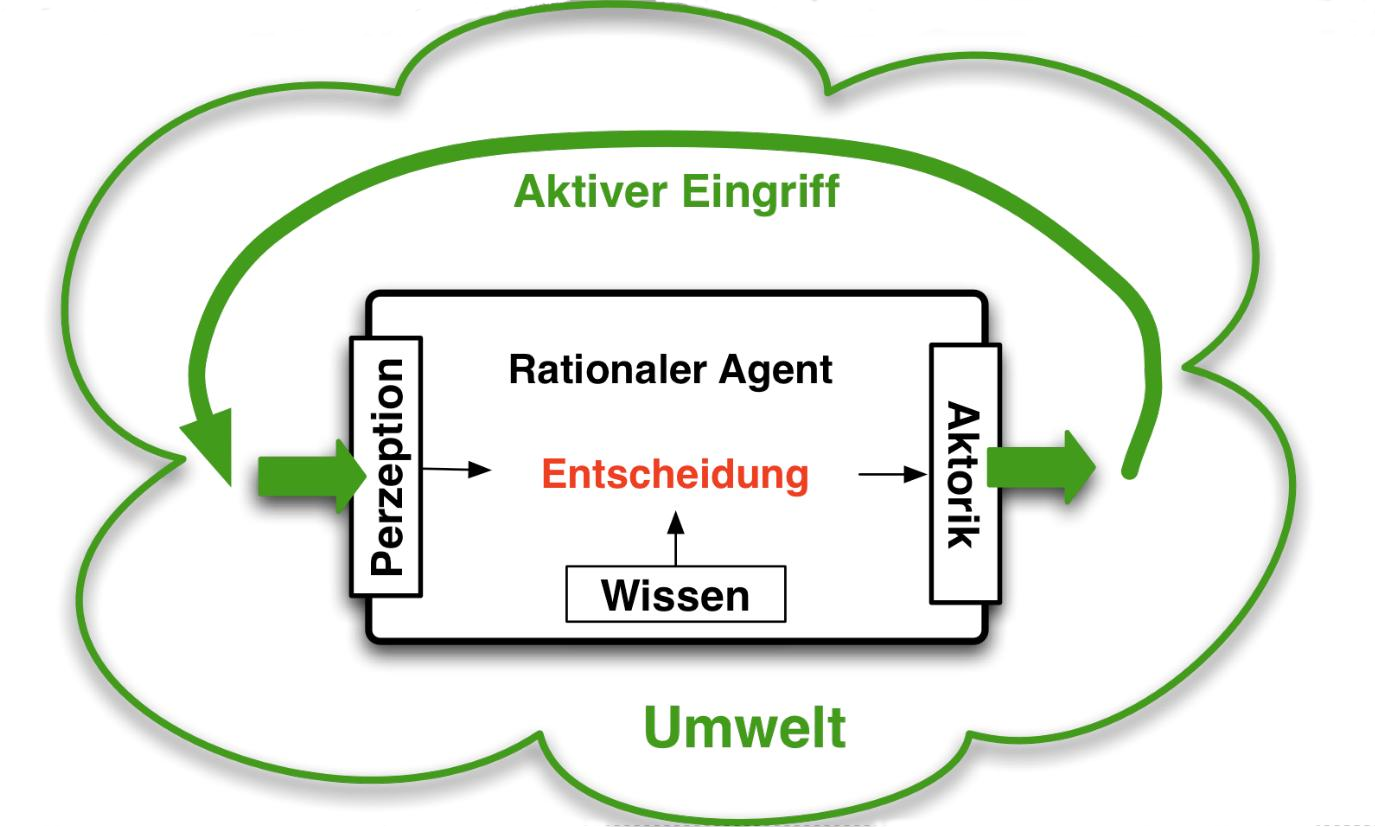
\includegraphics[width=0.8\textwidth]{figures/07_agentenzyklus.png}
\caption{Der Agentenzyklus}
\label{ch07_agentenzyklus}
\end{figure}

\subsubsection{Beispiele}
\paragraph{Schachcomputer}
\begin{itemize}
	\item Keine physische Umwelt
	\item Sehr beschränkte Umwelt
	\item Nur ein Ziel: das Spiel zu gewinnen
	\item Sensorik: Das Spielfeld wird komplette wahrgenommen
	\item Aktorik: Durchführung eines symbolischen Zugs
	\item Umwelt: semi-statisch, episodisch, diskret, deterministisch, vollständig beobachtbar, Multiagent
\end{itemize}
\paragraph{Industrieroboter}
\begin{itemize}
	\item oftmals, bei Abwesenheit von Sensorik, kein Agent, sondre nur ein Werkzeug
	\item Physische Umwelt
	\item Beschränkte Umwelt
	\item Wenn überhaupt rationaler Agent, üblicherweise extrem begrenzter Entscheidungsrahmen
	\item Ziel: Erfolgreiche Ausführung einer Operation
	\item Umwelt: dynamisch, episodisch, diskret oder kontinuierlich, deterministisch, vollständig beobachtbar, Einzelagent oder Multiagent
\end{itemize}
\paragraph{Mensch}
\begin{itemize}
	\item Extrem komplexe Umwelt
	\item Sehr mächtige Perzeption
	\item Sehr wissensbasiert
	\item Vielschichtige Motivationen und Zielsetzungen
	\item Umwelt: dynamisch, sequentiell, kontinuierlich, stochastisch, unvollständig beobachtbar, Multiagent
\end{itemize}
\paragraph{Serviceroboter}
\begin{itemize}
	\item Anforderungen dem Menschen viel ähnlicher als einem Industrieroboter
	\item Sehr komplexe Umwelt
	\item Vielschichtige Zielsetzung
	\item Es ist bei Servicerobotern ein ganz anderes Vorgehen, als bei Industrierobotern erforderlich
	\item Umwelt: wie beim Menschen
\end{itemize}

\subsubsection{Umwelt}
Für die verschiedenen Agenten werden sehr unterschiedliche Umgebungen benötigt.
Ein Rahmen für eine nützliche und eindeutige Charakterisierung von Umgebungen ist nötig.
\paragraph{Anforderungen}
\begin{itemize}
	\item Die Charakterisierung muss fundamentale, nicht oberflächliche Eigenschaften aufzeigen
	\item Es muss ein Rahmen gebildet werden, in den verschiedenen Verfahren und Paradigmen eingeordnet werden können
	\item eine Leitlinie für die Entwicklung neuer Verfahren muss gebildet werden
\end{itemize}
Umwelten verschiedener Agenten können gut durch einige fundamentale, duale Eigenschaften unterschieden werden.
\paragraph{Eigenschaften} \mbox{}
\vspace{1em} \\
\begin{tabular}{p{0.4\textwidth} p{0.1\textwidth} p{0.4\textwidth}}
\textbf{statisch} & \centering vs.\ & \textbf{dynamisch}\\
Der Agent ist das einzige Element, welches den Zustand der Umwelt verändert
& &
Die Umwelt kann sich auch ohne zutun des Agenten verändern
\\
\textbf{episodisch} & \centering vs.\ & \textbf{sequentiell}\\
Der zeitliche Verlauf des Geschehens  ist in abgeschlossene Einheiten unterteilt, zwischen denen keinerlei kausal Zusammenhänge bestehen
& &
Die vollständige zeitliche Vergangenheit hat Auswirkungen auf die Gegenwart ,die Gegenwart auf die gesamte Zukunft
\\
\textbf{diskret} & \centering vs.\ & \textbf{kontinuierlich}\\
Die Zustände der Umwelt sind diskret, ebenso der zeitliche Verlauf des Geschehens
& &
Der Zustandsraum der Umwelt ist kontinuierlich und die Zeit fließt ebenfalls kontinuierlich
\\
\textbf{deterministisch} & \centering vs.\ & \textbf{stochastisch}\\
Der Ausgang einer jeden Handlung ist eindeutig bestimmt
& &
Eine Handlung kann mit bestimmten Wahrscheinlichkeiten zu verschiedenen Ausgängen führen
\\
\textbf{vollständig} & \centering vs.\ & \textbf{unvollständig beobachtbar}\\
Der Agent kann die komplette Umwelt jederzeit vollständig und exakt wahrnehmen
& &
Der Agent kann die Umwelt nur eingeschränkt und fehlerbehaftet wahrnehmen
\\
\textbf{Einzelagent} & \centering vs.\ & \textbf{Multiagent}\\
Nur eine als Agent modellierbare Entität agiert in der Umwelt
& &
Viele als Agenten modellierbare Entitäten agieren in der Umwelt und können kooperieren oder konkurrieren
\end{tabular}

Die Beschreibung der Umwelt durch das jeweils komplexere Merkmal wird nur gewählt, wenn das einfachere Merkmal im Szenario des Agenten keine hinreichende Beschreibung ist.
Hinreichen ist hierbei auch in dem Sinne zu verstehen, dass es oftmals noch keine ausreichenden Verfahren gibt, um die komplexeren Merkmale zu berücksichtigen.

\subsubsection{Utility -- Motivation des Agenten}
\begin{itemize}
	\item Ein Agent benötigt Motivation um Absichten als Fundament für Entscheidungen
	\item In der Entscheidungstheorie durch das Konzept der \textbf{Utility} abgebildet (Ursprung des Begriffs in der Ökonomie)
	\item Dieses Konzept ist deutlich allgemeiner, als spezielle Ziele z.B.\ in der logikbasierten Planung	
\end{itemize}

\paragraph{Konzept}
\begin{itemize}
	\item Die utility modelliert in der Ökonomie ein numerisches Maß der Befriedigung eines Agenten (Menschen) durch einen bestimmten Konsum
	\item In der Robotik/KI wird jedoch ein Motivationsmaß eines Agenten nicht \emph{modelliert}, sondern \textbf{konstruiert}
	\item Die uitility wird hier genutzt, um einem künstlichen Agenten bestimmte Motivationen einzupflanzen
	\item Die utility ist ein allgemeines Konzept: es können konkurrierende und ergänzende Zielsetzungen fusioniert werden
	\item Im Rahmen der utility können auch Absichten gegeneinander abgewogen werden
\end{itemize}